\section{Contexte}

%
%\subsection{L'équipe}
%
%Mon stage s'est déroulé au sein de l'équipe Bonsai, équipe de recherche affiliée à l'Inria Lille - Nord Europe et le Centre de Recherche en Informatique, Signal et Automatique de Lille (CRIStAL, Université Lille 1, CNRS). 
%
%\subsubsection{Bonsai}
%L'équipe Bonsai compte 20 personnes, dont 10 membres permanents, sous la responsabilité d'Hélène Touzet. Le principal objectif de l'équipe est de développer des algorithmes d'analyse de séquences biologiques, que ce soit pour l'étude de l'ADN, de l'ARN, des protéines ou des NRP (peptides non-ribosomiques). Ce travail se réalise souvent en collaborations avec des biologistes, et se concrétise par la création de logiciels. Vidgil, par exemple, est une plate-forme  d'analyse des données de séquençage haut débit développée par l'équipe et utilisée à l'institut Pasteur pour suivre l'évolution de leucémies.
%


\subsection{Séquençage}
Le séquençage consiste à déterminer l'ordre des composants de molécules. Le séquençage de l'ADN sert à déterminer l'ordre des nucléotides composant un fragment donné. Pour cela, diverses techniques existent. Historiquement, la méthode la plus utilisée a été celle dite de Sanger, d'après son inventeur, plus facile à robotiser que celle de Maxam et Gilbert, développée à la même époque. Cependant, depuis quelques années, de nouvelles méthodes plus efficaces de séquençage haut débit sont apparues, multipliant le nombre de données issues du séquençage.

\subsubsection{Méthode de Sanger}
L'ADN polymérase est une enzyme utilisée dans la réplication de l'ADN, qui permet de créer des molécules d'ADN en assemblant des nucléotides. Les nucléotides utilisés lors de la réplication sont des désoxyribonucléotides (dNTP), mais il existe aussi des didésoxyribonucléotides (ddNTP), qui forcent l’arrêt de la réaction à la suite de leur utilisation. 

La méthode de Sanger consiste à répliquer un brin d'ADN dans un milieu ou se trouvent des dNTP ainsi que de quelques ddNTP d'un seul type (ddnTP à Guanine, Thymine, Adénine ou Cytosine). La réplication va donc s’arrêter aléatoirement sur l'un des nucléotides correspondant à la ddNTP choisie. Cette expérience est répétée quatre fois, avec les quatre types de ddNTP, puis l'on compare les longueurs des brins d'ADN répliqués par chromatographie.


\begin{figure}[!ht]
    \center
    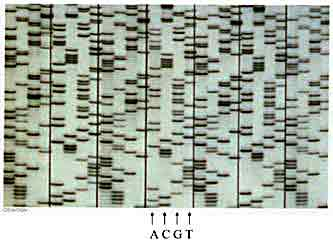
\includegraphics[]{./images/chromato_acanthoweb.jpg}
    \caption{Exemple de chromatographie}
    \label{chromato}
\end{figure}


Il ne reste plus qu'à lire la séquence ADN, processus automatisable mais long.

\subsubsection{Séquençage haut débit}
Il existe de nombreuses techniques de séquençage haut débit, plus ou moins chères, fiables ou efficaces.
Par exemple, le séquençage par synthèse, utilisé par l'entreprise \emph{Illumina}, est basé sur l'utilisation de colorants fluorescents.

Pour cette méthode, on attache aux séquences étudiées des amorces, qui servent à la synthèse de l'ADN. Puis avec l'ajout de nucléotides et d'ADN polymérase, ces séquences sont amplifiées. On ajoute enfin des nucléotides associés à des couleurs spécifiant leur type (Guanine, Thymine, Cytosine et Adénine), qui vont s'associer à leur complémentaire sur les brins d'ADN. Les nucléotides non-attachés sont ensuite enlevés, et les colorants excités et photographiés. Les colorants sont retirés chimiquement et le processus répété plusieurs fois jusqu'à ce que l'ensemble de l'ADN soit séquencé.

\subsubsection{Reads}
Les données retournées par les séquenceurs sont appelées des \emph{reads}. Ce sont de très nombreux fragments de l'ADN séquencé. La taille et le nombre de ces fragments varient, mais ils sont souvent composés de 100 à 300 nucléotides et couvrent au moins 30 à 40 fois la séquence initiale. 

Ce sont donc des données très redondantes, ce que nous chercherons à exploiter dans ce stage.


\subsection{Structures de données utilisées}

\subsubsection{Tableau de suffixe}
Un suffixe d'une chaîne de caractères $s$ est une chaîne $s'$ plus petite tel que $s'$ termine $s$. C'est-à-dire tel qu'il existe une chaîne $p$, pouvant être vide, telle que $p + s' = s$, avec $+$ représentant la concaténation des chaînes. $p$ est d'ailleurs un préfixe de $s$.

Un tableau de suffixes est un tableau d'entiers représentant tous les suffixes d'une chaîne. Pour le construire, il faut construire l'ensemble des suffixes, en attribuant à chaque suffixe un entier présentant son ordre dans le texte. Les suffixes sont ensuite triés par ordre lexicographique, et seuls leur place est gardée. La figure \ref{suffixes} illustre cette construction.

\begin{figure}[h!]
\fbox{%
  \begin{minipage}{0.4\linewidth}
  	\begin{flushleft}
      \textsc{%
  	  \begin{tabular}{l|c|}
  	  	suffixe & indice \tabularnewline \hline
        barbapapa\$ & 0\\
	    arbapapa\$ & 1\\
	    rbapapa\$ & 2\\
	    bapapa\$ & 3\\
	    apapa\$ & 4\\
	    papa\$ & 5\\
	    apa\$ & 6\\
	    pa\$ & 7\\
        a\$ & 8\\
	    \$ & 9
	  \end{tabular} 
	  }
  	\end{flushleft}
  \end{minipage}%
  \begin{minipage}{0.2\linewidth}
	\begin{center}
		tri\\
  		$\rightarrow$
	\end{center}
  \end{minipage}%
  \begin{minipage}{0.4\linewidth}
  	\begin{flushright}
      \textsc{%
  	  \begin{tabular}{|l|c}
  	  	suffixe & indice\tabularnewline \hline
	    \$ & {\color{red}9}\\
        a\$ & {\color{red}8}\\
	    apa\$ & {\color{red}6}\\
	    apapa\$ & {\color{red}4}\\
	    arbapapa\$ & {\color{red}1}\\
	    bapapa\$ & {\color{red}3}\\
	    barbapapa\$ & {\color{red}0}\\
	    pa\$ & {\color{red}7}\\
        papa\$ & {\color{red}5}\\
	    rbapapa\$ & {\color{red}2}\\
	  \end{tabular} 
	  }
  	\end{flushright}
  \end{minipage}%
}
\caption{Construction du tableau des suffixes (en rouge) pour la chaîne "\textsc{barbapapa\$}"}
\label{suffixes}
\end{figure}

\subsubsection{Wavelett tree}
Les arbres sont des structures de données couramment utilisés en informatique, représentant des graphes acycliques orientés, tels que tous les nœuds sauf un, la racine, ont un unique parent. Pour les arbres binaires, comme le wavelett tree, les nœuds ont au plus deux fils. Les nœuds n'ayant pas de fils sont appelés feuilles.

Le \textit{wavelett tree}, ou arbre d'ondelettes, est une structure de données succincte (c'est-à-dire compressée presque optimalement), à l'origine utilisée pour représenter les tableaux de suffixes compressés.

La construction du wavelett tree est basée sur la division de l'alphabet du mot d'origine en deux. Cette division peut se faire par ordre lexicographique, ou par d'autres algorithmes plus complexes tels que le codage de Huffman. Nous ne nous intéresserons ici qu'à la première façon.

Prenons comme exemple la construction du wavelett tree de \textsc{"barbapapa\$"}. L'alphabet est l'ensemble \textsc{{'\$'; 'a'; 'b'; 'p'; 'r'}}. Les lettres appartenant à la première moitié de l'alphabet (\textsc{{'\$'; 'a'}}) seront représentées par un 0, tandis que les lettres de la deuxième moitié seront des 1. La racine comporte donc le mot "1011010100".

Les deux moitiés de l'alphabet descendent dans les fils de la racine. Le premier nœud code donc \textsc{"aaaa\$} sur l'alphabet \textsc{{'\$'; 'a'}}, et le deuxième nœud code \textsc{"brbpp"} sur l'alphabet \textsc{{'b'; 'r';p}}. La même opération que sur la racine est alors renouvelée, jusqu'à ce que les nœuds ne codent plus qu'une seule lettre.

%Exemple

\subsection{Transformée de Burrows-Wheeler}

La transformée de Burrows-Wheeler\up{\cite{bwt}}, abrégée \bwt, est un algorithme de réorganisation des données  fréquemment utilisé pour compresser les données. Elle est réversible, augmente la probabilité que des caractères identiques se retrouvent à côté. Il est notamment utilisé dans l'algorithme de compression \emph{bzip2}. 

\subsubsection{Construction}
La construction de la \bwt\ est simple : elle consiste à prendre la dernière lettre de toutes les rotations de la chaîne initiale triées lexicographiquement.
Une rotation de $k$ éléments d'une chaîne de caractères de longueur $n$ est composée des $n-k$ derniers éléments de la chaîne concaténés aux $k$ premiers.
Ainsi, on peut voir l'ensemble des rotations d'une chaîne de caractères "\textsc{barbapapa\$}" dans la figure \ref{rotations}.

\begin{figure}[h!]
\fbox{%
  \begin{minipage}{\linewidth}
  	\begin{center}
 \textsc{%
      barbapapa\$\\
	  arbapapa\$b\\
	  rbapapa\$ba\\
	  bapapa\$bar\\
	  apapa\$barb\\
	  papa\$barba\\
	  apa\$barbap\\
	  pa\$barbapa\\
      a\$barbapap\\
	  \$barbapapa
	  }
	\end{center}
  \end{minipage}%
}
\caption{Ensemble des rotations de la chaîne "\textsc{barbapapa\$}"}
\label{rotations}
\end{figure}

Ordonnés par ordre lexicographique, on obtient l'exemple \ref{bwt}, où l'on ne garde que la dernière lettre pour avoir la \bwt.
\begin{figure}[h!]
\fbox{%
  \begin{minipage}{\linewidth}
    t = "\textsc{barbapapa\$}"
  	\begin{center}
  	  \textsc{%
      \$barbapap {\color{red}a}\\
      a\$barbapa {\color{red}p}\\
	  apa\$barba {\color{red}p}\\
	  apapa\$bar {\color{red}b}\\
	  arbapapa\$ {\color{red}b}\\
	  bapapa\$ba {\color{red}r}\\
	  barbapapa {\color{red}\$}\\
	  pa\$barbap {\color{red}a}\\
	  papa\$barb {\color{red}a}\\
	  rbapapa\$b {\color{red}a}
	  }
	\end{center}
	\bwt(t) = "\textsc{appbbr\$aaa}"
  \end{minipage}%
}
\caption{Construction de la \bwt\ de "\textsc{barbapapa\$}"}
\label{bwt}
\end{figure}

On peut d'ailleurs remarquer les suites de P, B et A. En effet, lorsque les lettres sont suivies des mêmes caractères, elles vont se retrouver à côté dans la \bwt, facilitant ainsi la compression.

\subsubsection{Réversibilité}
Lorsqu'un algorithme est réversible, c'est que l'on peut retrouver sa donnée de départ à partir de son résultat. C'est donc une propriété importante de la \bwt, puisqu'elle permet de retrouver le texte de départ.

Pour assurer la réversibilité de la \bwt, on ajoute un caractère spécial, lexicographiquement plus petit que tous les autres et traditionnellement représenté par \$. Ainsi, on est assuré de savoir où se termine la chaîne initiale.

Pour inverser la \bwt, on reconstruit le tableau des rotations, colonne par colonne.
Tout d'abord, la dernière colonne correspond à la \bwt, et la première à l'ensemble des lettres dans l'ordre lexicographique. Comme ce sont des rotations, les lettres de la première colonne suivent celles de la dernière. En triant ces groupes de deux lettres, on obtient donc la deuxième colonne, comme dans la figure \ref{unbwt}

\begin{figure}[h!]
\fbox{%
  \begin{minipage}{\linewidth}
	\bwt(t) = "\textsc{appbbr\$aaa}"
  	\begin{center}
  	  \textsc{%
      \$b . . . . . . a{\color{lightgray}\$}\\
	  a\$ . . . . . . p{\color{lightgray}a}\\
	  ap . . . . . . p{\color{lightgray}a}\\
	  ap . . . . . . b{\color{lightgray}a}\\
	  ar . . . . . . b{\color{lightgray}a}\\
	  ba . . . . . . r{\color{lightgray}b}\\
	  ba . . . . . . \${\color{lightgray}b}\\
	  pa . . . . . . a{\color{lightgray}p}\\
	  pa . . . . . . a{\color{lightgray}p}\\
	  rb . . . . . . a{\color{lightgray}r}
	  }
	\end{center}
  \end{minipage}%
}
\caption{Inversion de la \textsc{bwt} | Construction de la deuxième colonne}
\label{unbwt} 
\end{figure}

On construit de la même façon les colonnes suivantes, pour lire la chaîne initiale sur la ligne terminant par \$.

\subsubsection{FM-index}

En 2000, Paolo Ferragina et Giovanni Manzini créent une structure d'indexation, appelée FM-index, basée sur la \bwt. 

Le FM-index contient la \bwt, un échantillonnage du tableau des suffixes (qui donne la position dans le texte initial de chaque rotation), ainsi qu'une fonction $rank(c, i)$  et un tableau $C$.
La fonction $rank(c, i)$ renvoie  le nombre de caractère $c$ dans $\bwt[0..i]$. Le tableau $C$ donne pour chaque caractère de \bwt\ le nombre de caractère lexicographiquement plus petit que lui.

Grâce à cette structure, il est possible de calculer le mappage entre la \bwt\ (dernière colonne de la table des rotations, aussi désignée par L pour \textit{last}) et la première colonne de la table des rotations (désignée par F pour \textit{first}). Ce mappage, appelé fonction LF() est montré dans la figure \ref{lf}.

L'inversion de la \bwt\ peut se faire avec LF() sans la reconstruction de la totalité du tableau des rotations. 
Il suffit de partir de \$ et de remonter la fonction LF(), en reconstruisant la chaîne initiale jusqu'au début.

Par exemple, dans la figure \ref{lf}, '\$' est à l'indice 6, et LF(6) = 0. \bwt[0] = \textsc{'a'}, donc t se termine par \textsc{"a\$"}. On continue, LF(0) = 1, t = \textsc{"...pa\$"} ; LF(1) = 7, t = \textsc{"...apa\$"} ; ainsi de suite jusqu'à ce qu'on ai retrouvé l'entièreté de la chaîne de départ.

\begin{figure}[h!]
\fbox{%
  \begin{minipage}{\linewidth}
	\bwt(t) = "\textsc{appbbr\$aaa}"
  	\begin{center}
  	  \textsc{%
  	  \begin{tabular}{c|c|c}
  	  	\textup{i} & \bwt & \textsc{LF(\textup{i})}\tabularnewline \hline
        0 & \$barbapap {\color{red}a} & 1 \\
	    1 & a\$barbapa {\color{red}p} & 7 \\
	    2 & apa\$barba {\color{red}p} & 8 \\
	    3 & apapa\$bar {\color{red}b} & 5 \\
	    4 & arbapapa\$ {\color{red}b} & 6 \\
	    5 & bapapa\$ba {\color{red}r} & 9 \\
	    6 & barbapapa {\color{red}\$} & 0 \\
	    7 & pa\$barbap {\color{red}a} & 2 \\
	    8 & papa\$barb {\color{red}a} & 3 \\
	    9 & rbapapa\$b {\color{red}a} & 4
  	  \end{tabular}	
	  }
	\end{center}
  \end{minipage}%
}
\caption{La fonction LF()}
\label{lf} 
\end{figure}

Grâce à cette structure, Ferragina et Manzini développent également un nouvel algorithme, appelé \textit{backward search}, qui émule sur la \bwt\ la recherche dans un tableau de suffixe.

Pour trouver un motif $m$, on commence par regarder la dernière lettre de $m$, qu'on appellera $a$. Les rotations commençant par cette lettre se trouvent entre les indices $s_a = C[a] + 1$ et $e_a = C[succ(a)]$, avec $succ(a)$ la fonction qui renvoie la lettre suivant $a$ dans l'alphabet. 

Puis, on prend l'avant dernière lettre de $m$, désignée par $b$. Cette fois, le préfixe $ba$ est trouvé dans les rotations $s_b = C[b] + Occ(b, s_a-1) + 1$ et $e_b = C[b] + Occ(b, e_a)$.

On répète cette opération jusqu'à ce qu'on ai trouvé l'ensemble des rotations dont $m$ est préfixe, ou que les bornes $s_x$ et $e_x$ se rejoignent ou se croisent. Si $e_x - s_x \le 0$, alors $m$ n'est pas dans le texte.

Une fois ces bornes délimitées, on utilise le tableau de suffixes pour trouver les positions de $m$ dans le texte. Soit $p$ l'échantillonnage du tableau de suffixe SA, la position des préfixes des rotations $r$ multiples de $p$ dans le texte est SA[$r/p$]. Pour les rotations qui ne sont pas multiples de $p$, on parcourt la fonction LF() jusqu'à trouver l'une de ces rotations. La position de $m$ se retrouve en ajoutant à la position de cette rotation le nombre de fonction LF() calculées pour y parvenir.
%Exemple

\subsubsection{Contexte borné}
Un inconvénient majeur de la \bwt\ est le temps et l'espace nécessaires à sa construction. En effet, trier les rotations peut prendre au maximum $n^{2}$ comparaisons, $n$ étant la longueur de la chaîne.
Pour pallier à cela, Shindler en 1997 et Yoko en 1999 proposent de ne trier les suffixes que jusqu'à un rang $k$. 

Cette nouvelle structure est couramment appelée transformée de Burrows-Wheeler à contexte borné, ou $k$-\bwt, et on appelle $k$-contextes les parties de la \kbwt\ dont les rotations sont égales jusqu'à $k$. Dans ces $k$-contextes, les rotations sont rangées dans l'ordre d'apparition dans le texte. L'information de ces $k$-contextes peut être stockée dans un vecteur de bit, que nous appellerons ici $Dk$. Elle peut aussi être retrouvée en temps voulue, comme décrit par Matthias Pétri\up{\cite{petri}} dans sa thèse.

Le résultat de la \kbwt\ est très proche de la \bwt\ lorsque $k$ est petit, puisque les deux chaînes ne diffèrent que sur les $k$-contextes. La \kbwt\ est donc également compressible facilement.

Pour inverser la \kbwt, on utilise on utilise la fonction LF() de la même façon que dans le FM-index pour les k-contextes de taille 1. Lorsque LF() pointe sur un contexte plus grand, les $k$-contextes étant déjà dans l'ordre du texte, il suffit de prendre la première lettre, et de marquer le début du contexte à la lettre suivante.
%Exemple

Si la fonction LF() ne mappant pas exactement la première et dernière colonne n'est pas un problème pour la réversibilité de la \kbwt, elle empêche en revanche la \textit{backward search}. Petri\up{\cite{petri}} a donc 
trouver un algorithme pour retrouver LF() à partir de la \kbwt, la $k-1$-\bwt, et quelques structures auxiliaires.
